\chapter{Authentication Mechanisms}
\label{cha:authentication_mechanisms}
This chapter explains the concepts and mechanisms of the discussed authentication mechanisms.
Only the mTLS and and the JWT approach are discussed, since the TTN approach is deprecated and should not be used anymore~\cite{dias2020microservices}.
Furthermore this chapter clarifies the advantages and disadvantages of the discussed mechanisms.

\begin{figure}
	\centering
	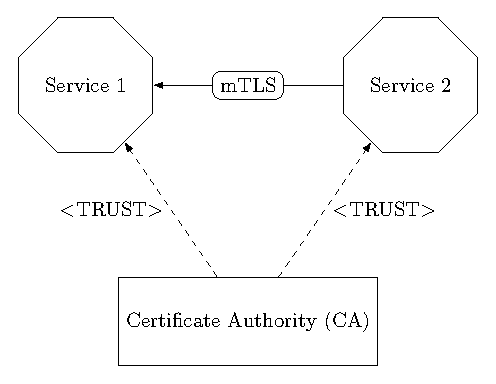
\includegraphics{images/authentication-mechanisms/TikZ_mTLS_base_structure.pdf}
	\caption{Setup using mTLS for the service-to-service authentication~\cite{dias2020microservices}}
	\label{fig:auth_mechanisms_mtls}
\end{figure}

\section{Authentication based on mTLS}
Mutual TLS is the most popular option for the service-to-service authentication of microservice deployments~\cite{dias2020microservices}.
Securing the communication with TLS already provides integrity, confidentiality and furthermore authenticates the server to the client.
Since basic TLS does not provide authentication from the client to the server, it is not sufficient for the service-to-service security.
Therefore mutual TLS is used, which provides an efficient and straightforward approach to authenticate the client to the server.

The authentication using mTLS requires a PKI, same as the authentication using basic TLS.
It is possible to use the already existing PKI of the internet, but this would make the key management much harder and would not bring any advantages.
% TODO: Insert Reference to self hosted PKI
Therefore it is good practise to use a self-hosted PKI to have a root of trust within the network~\cite{dias2020microservices}.
The setup of a microservice deployment using mTLS is shown in figure~\ref{fig:auth_mechanisms_mtls}.

When mTLS is used, both the server and the client must provide a valid certificate to create a communication channel.
The issuer of the presented certificates must be trusted by all communicating parties~\cite{dias2020microservices}.
If one communication partner does not have a valid certificate which is signed by a trusted issuer, the communication is neglected.
Therefore each service needs a private key, a public key.
Additionally a signed certificate, which binds the public key to the subject of the certificate, is needed.
The certificates of the communication partners are exchanged during the TLS handshake.

\subsection{Handshake}
\label{sec:tlshandshake_details}
The handshake is used exchange the the certificates of the server and the client.
The steps of the handshake differ between the used algorithms and versions of the TLS protocol.
The following sequence should give an overview about the steps of the TLS handshake using mutual TLS~\cite{parsovs2013practical}.
The sequence is visualized in figure~\ref{fig:tlshandshake}.
\begin{enumerate}
	\item The client initializes the connection by sending a \textbf{ClientHello} message to the server.
		The \textbf{ClientHello} message includes a list of supported cipher suits, and the randomness, which is a combination of random bytes and the current date~\cite{mediumtls}.
	\item The sever responds with a \textbf{ServerHello}, in which the server chooses one cipher suite of the \textbf{ClientHello} message.
		Furthermore the \textbf{ServerHello} contains the servers randomness.
	\item The server sends the \textbf{Certificate} messages, containing one or more certificates, which can be used to build the chain.
		The client validates the sent certificates with his own trusted store.
		If the trusts the sent certificate chain, the server is authenticated successfully.
	\item The server sends the \textbf{CertificateRequest} message, in which the trusted CAs of the server are listed.
		The client can use this list to choose the correct certificate he has to present.
	\item The server sends the \textbf{ServerHelloDone} message.
	\item The client responds with his \textbf{Certificate} message, which is similiar to the servers \textbf{Certificate} message, but contains the client's certificate.
	\item The client he generates a random value the pre-master secret, which is used to derive symmetric keys for the cipher suite.
		The pre-master secret is then encrypted, using the public key of the server.
		The public key of the server is assumed to be the first certificate of the \textbf{Certificates} message by the server.
		The encrypted pre-master secret is then transferred to the server within the \textbf{ClientKeyExchange} message.
	\item The client has to proove the client that he owns the corresponding private key of the sent certificate.
		Therefore he has to encrypt the hash of all previous messages with his private key.
		This encrypted hash is then sent to the server within the \textbf{CertificateVerify} message.
		The sever can decrypt the hash with the public key of the certificate and can calculate the hash on his own to check whether the decrypted hash is correct or not.
	\item The client sends a \textbf{ChangeCipherSpec} message, to signal the server, that all following messages will be protected with the protection mechanisms defined in the cipher suite.
	\item The last message of the handshake is the \textbf{Finished} message, which is an encrypted hash of all previous messages.
\end{enumerate}

\begin{figure}
    \centering
	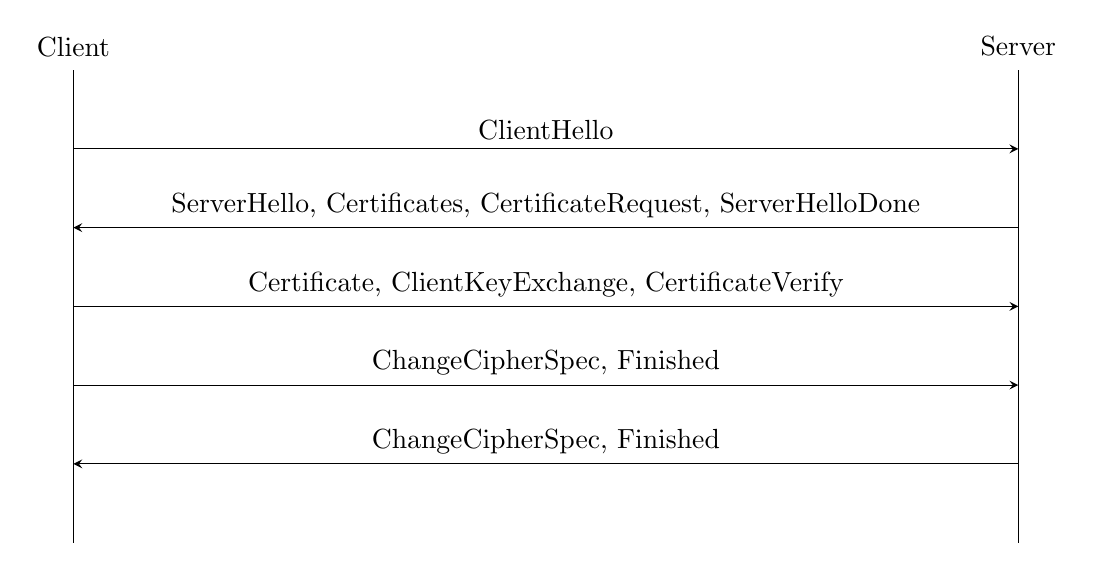
\begin{tikzpicture}
		\draw (-6,0) -- (-6,-6) (6,0) -- (6,-6);
		\node at (-6,.3) {Client};
		\node at (6,.3) {Server};

		\draw[-stealth] (-6,-1) -- node[midway,above] {ClientHello} (6,-1);
		\draw[stealth-] (-6,-2) -- node[midway,above] {ServerHello, Certificates, CertificateRequest, ServerHelloDone} (6,-2);
		\draw[-stealth] (-6,-3) -- node[midway,above] {Certificate, ClientKeyExchange, CertificateVerify} (6,-3);
		\draw[-stealth] (-6,-4) -- node[midway,above] {ChangeCipherSpec, Finished} (6,-4);
		\draw[stealth-] (-6,-5) -- node[midway,above] {ChangeCipherSpec, Finished} (6,-5);
	\end{tikzpicture}
    \caption{TLS handshake using mTLS~\cite{parsovs2013practical}}
    \label{fig:tlshandshake}
\end{figure}
